\documentclass[sigconf]{acmart}

\usepackage[utf8]{inputenc}
\usepackage{booktabs} % For formal tables
\usepackage{algorithmicx}
\usepackage{algpseudocode}
\usepackage{algorithm}
\usepackage[inline]{enumitem}
\usepackage{varwidth}

%\usepackage{todonotes}
\usepackage{graphicx}
\graphicspath{figures}
\usepackage{svg}

\def\xcolorversion{2.00}
\def\xkeyvalversion{1.8}

\usepackage{pgf}
\usepackage{tikz}
\usetikzlibrary{arrows,shapes,snakes,automata,backgrounds,petri}

\newcommand\note[2]{{\color{#1}#2}}
\newcommand\todo[1]{{\note{red}{TODO: #1}}}

\newcommand*{\fullref}[1]{\hyperref[{#1}]{\autoref*{#1} (\nameref*{#1})}} % One single link

% Adds a "given" symbol (vertical bar) that rescales in height (like \left and \right)
\usepackage{mathtools}
\newcommand\givenbase[1][]{\:#1\lvert\:}
\let\given\givenbase
\newcommand\sgiven{\givenbase[\delimsize]}
\DeclarePairedDelimiterX\Basics[1](){\let\given\sgiven #1}
\newcommand\Average{E\Basics}

\makeatletter
\newcommand{\StateIndent}[1][3]{%
  \setlength\@tempdima{\algorithmicindent}%
  \Statex\hskip\dimexpr#1\@tempdima\relax}
\algdef{S}[WHILE]{WhileNoDo}[1]{\algorithmicwhile\ #1}%
\makeatother

\algnewcommand\True{\textbf{true}}
\algnewcommand\False{\textbf{false}}
\algnewcommand\Break{\textbf{break}}

\newcommand{\algorithmautorefname}{Algorithm}

% Copyright
%\setcopyright{none}
%\setcopyright{acmcopyright}
%\setcopyright{acmlicensed}
\setcopyright{rightsretained}
%\setcopyright{usgov}
%\setcopyright{usgovmixed}
%\setcopyright{cagov}
%\setcopyright{cagovmixed}

% DOI
\acmDOI{10.475/123_4}

% ISBN
\acmISBN{123-4567-24-567/08/06}

%Conference
\acmConference[WOODSTOCK'97]{ACM Woodstock conference}{July 1997}{El
  Paso, Texas USA} 
\acmYear{2017}
\copyrightyear{2017}

\acmPrice{15.00}


\begin{document}
\title{TCP Rax: Deep Reinforcement Learning for TCP Congestion Control}
\titlenote{Produces the permission block, and
  copyright information}
%\subtitle{Extended Abs\texttt{tract}
%\subtitlenote{The full version of the author's guide is available as
%  \texttt{acmart.pdf} document}}

%\author{Maximilian Bachl} 
%\affiliation{%
% \institution{Institute of Telecommunications}
% \streetaddress{Gußhausstraße 25}
% \postcode{1040}
% \city{Vienna} 
% \country{Austria}}
%\email{maximilian.bachl@tuwien.ac.at}
%
%\author{Tanja Zseby} 
%\affiliation{%
% \institution{Institute of Telecommunications}
% \streetaddress{Gußhausstraße 25}
% \postcode{1040}
% \city{Vienna} 
% \country{Austria}}
%\email{tanja.zseby@tuwien.ac.at}
%
%\author{Joachim Fabini} 
%\affiliation{%
% \institution{Institute of Telecommunications}
% \streetaddress{Gußhausstraße 25}
% \postcode{1040}
% \city{Vienna} 
% \country{Austria}}
%\email{joachim.fabini@tuwien.ac.at}

% The default list of authors is too long for headers}
%\renewcommand{\shortauthors}{Bachl, Zseby, Fabini}

\begin{abstract}

A major challenge in congestion control is to find a set of rules that dynamically adapt the congestion window to current and anticipated future network conditions to maximize a specified utility function, e.g. maximum throughput or minimum packet loss. 

This paper proposes Reactive Adaptive eXperience based congestion control (TCP Rax), a new method of congestion control that uses online reinforcement learning to maintain an optimum congestion window with respect to a given utility function. We use a neural network based approach that can be initialized either with random weights (without prior knowledge) or with a previously trained neural network to improve stability and convergence time. The processing of rewards in congestion control depends on the arrival of acknowledgments, inducing loop delays that may lead to oscillations. As a remedy we propose a specific formulation of neural network based reinforcement learning that supports the proactive processing of delayed and partial rewards. 

We show that our method converges to a stable, close-to-optimum solution within the order of minutes and outperforms existing congestion control algorithms in typical networks. Thus, this paper demonstrates that neural network based reinforcement learning without any prior knowledge can feasibly be done on-line and can compete with human-designed congestion-control schemes such as New Reno and Cubic.

\end{abstract}

%
% The code below should be generated by the tool at
% http://dl.acm.org/ccs.cfm
% Please copy and paste the code instead of the example below. 
%
\begin{CCSXML}
<ccs2012>
<concept>
<concept_id>10003033.10003039.10003048</concept_id>
<concept_desc>Networks~Transport protocols</concept_desc>
<concept_significance>500</concept_significance>
</concept>
<concept>
<concept_id>10003752.10010070.10010071.10010261.10010275</concept_id>
<concept_desc>Theory of computation~Multi-agent reinforcement learning</concept_desc>
<concept_significance>500</concept_significance>
</concept>
<concept>
<concept_id>10010520.10010521.10010542.10010294</concept_id>
<concept_desc>Computer systems organization~Neural networks</concept_desc>
<concept_significance>300</concept_significance>
</concept>
</ccs2012>
\end{CCSXML}

\ccsdesc[500]{Networks~Transport protocols}
\ccsdesc[500]{Theory of computation~Multi-agent reinforcement learning}
\ccsdesc[300]{Computer systems organization~Neural networks}

\keywords{congestion control, machine learning, reinforcement learning, artificial neural networks}

\settopmatter{printfolios=true}

\maketitle%

\section{Introduction}

Recent advances in neural network based reinforcement learning (RL) raise the question if it is possible to use these frameworks to model end-to-end congestion control. In general, in congestion control each sender aims to maximize an objective function that usually comprises of
\begin{enumerate*}
\item sending as many packets as possible
\item with as little delay as possible
\item while minimizing the amount of lost packets
\end{enumerate*}. As, for instance, for some applications overall throughput is more important than little packet loss, each application can define its preference using a custom utility function. Clearly, it is also desirable from an overall point of view that all senders use available resources in a way that is fair to the others: When several senders share an Internet link under the same conditions, they should receive an equal share of the reward. To achieve fairness, it is necessary that senders only use utility functions that 
\begin{enumerate*}
\item converge to a stable equilibrium and
\item provide each sender with a fair share of his subgoals
\end{enumerate*}. 

In an ideal machine learning based congestion control method, each sender uses a set of observed environment conditions to determine which action he should take to maximize his reward in the future. The environment conditions can be any metrics that the sender can obtain from the network, for example the mean round-trip time of the last received packets, the packet loss rate etc. An action is a change to the sending rate: For example, if a sender perceives an increase in the loss rate it might be advisable to lower the sending rate. To modulate the sending rate one can  either
\begin{enumerate*}
\item change the sending rate itself at certain points in time or
\item maintain a congestion window that indicates the number of packets that can be in flight at a certain point in time
\end{enumerate*}. It seems preferable to maintain a congestion window, as one cannot be certain that the operating system (OS) can maintain a certain constant sending rate for each application on one machine, as the OS has to schedule different applications and share the network interfaces between them. 

While congestion control seems to be a well suited problem for reinforcement learning, there are a couple of challenges and differences from most other reinforcement learning problems:  \begin{itemize}
\item For instance, when playing a video game, if one pushes a button, one can see the consequences of an action immediately. However, in congestion control, the rewards are always \textbf{delayed} by one round-trip time.
\item Due to the delay, by the time an action receives its reward, probably other actions have already been carried out in the meantime. Thus, contrary to classical RL, \textbf{action and rewards are not synchronized}. 
\item \textbf{Actions and rewards are not atomic}: If an action causes three packets to be sent, we consider these three packets being sent three \textit{partial actions}. In case these packets are transmitted correctly, the receiver will send back three acknowledgements. Each of these acknowledgements is a \textit{partial reward} that already unveils new information on the current state of the network and enables the sender to take an action based on this new information. However, only if all partial rewards have been received, the sender can assemble the overall reward of the corresponding action and can perform an update of the underlying reinforcement learning logic. 
\item The \textbf{number of actions and rewards} per unit of time is \textbf{variable}: If the congestion window is larger, more packets are sent and more acknowledgements are received, which means that the reinforcement learning algorithm gets more training data the larger the window is. This is problematic as it means that -- without proper adjustments -- the experience made at a larger congestion window will ``overwrite'' the experience made at a smaller window as with the larger window simply more training data arrives and it is thus going to be overemphasized. 
\end{itemize}

To address these problems, we develop a new formulation of reinforcement learning called \textit{Partial Action Learning} (PAL). PAL is a superset of reinforcement learning: If one uses PAL for a learning problem without delay, asynchronicity and partial actions/partial rewards, one gets classical reinforcement learning.

While using PAL to train an optimum congestion control for a specific range of network scenarios in an off-line fashion is possible, it is something that has already been done previously in an approach called \textit{Remy} \citep{winstein_tcp_2013}. The only potential advantage that PAL could provide here is increased training speed. Thus, we want to show that it is  not only possible to learn congestion control by using machine learning but that it is even possible to do so on-line and without any preknowledge about the network environment.

Using a utility function that encourages high throughput and discourages packet loss (adapted from \citep{dong_pcc:_2015}) we see that our machine learning approach can learn congestion control that maximizes this objective given a couple of minutes of time (without any pre-training) \ref{fig:demo}. 

\begin{figure}
\begin{minipage}{\columnwidth}
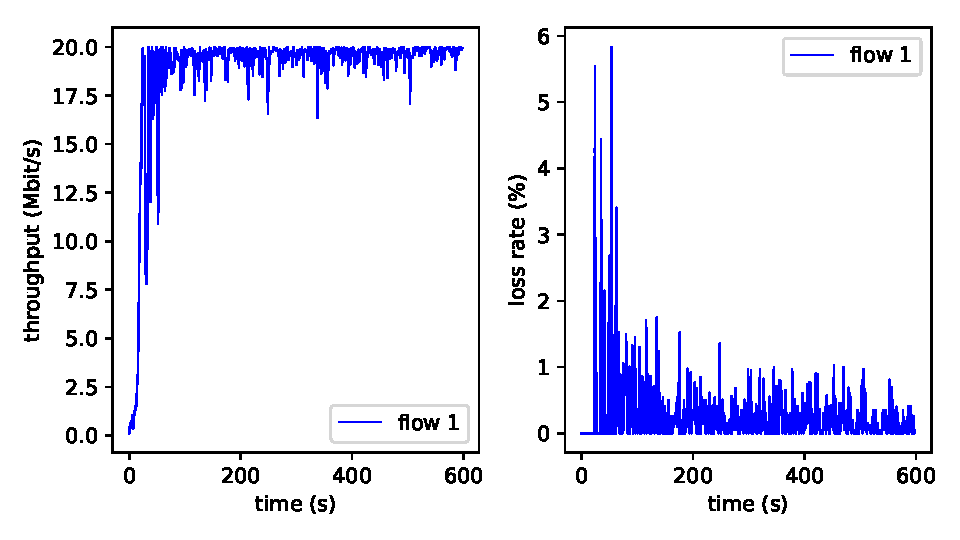
\includegraphics[width=\columnwidth]{{{/home/max/repos/remy/compute-0-4.local/figures/4_1_2018-01-25-20:17:15_3_2018-01-25-20:17:15.0}}}
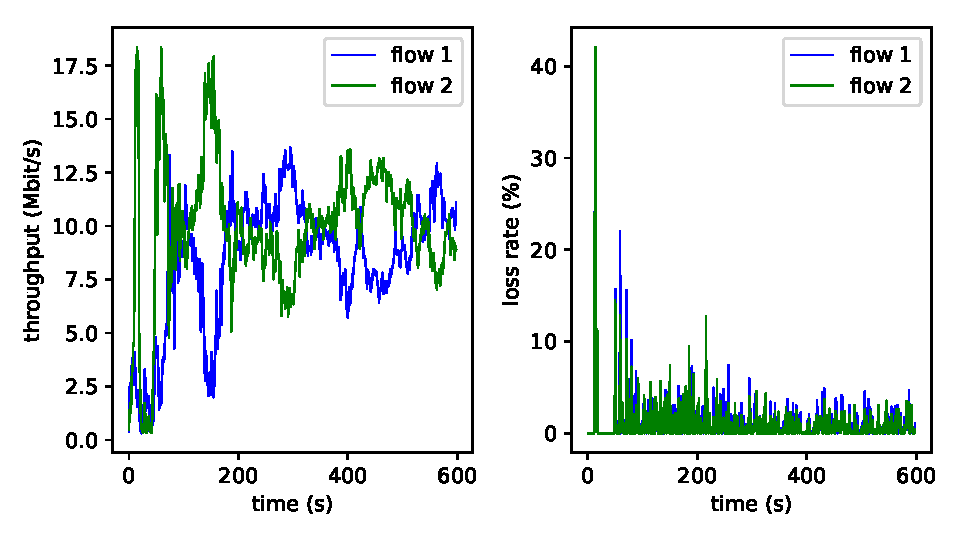
\includegraphics[width=\columnwidth]{{{/home/max/repos/remy/compute-0-6.local/figures/4_2_2018-01-25-19:53:39_22_2018-01-25-19:53:39.0}}}
\caption{The throughput and the loss rate when sharing a bottleneck link of 20\,Mbit/s with a two-way end-to-end delay of 50\,ms and a very small buffer of $\frac{1}{10}$ bandwidth delay product between 1 and 2 senders (from top to bottom). The time needed for convergence increases with more senders, which is caused by the fact that the more senders use the link, the fewer because each sender receives fewer packets per unit of time for training and because the environment gets more complex. It is interesting to note that in the case of two senders, both flows complement each other and quickly adapt to the sending rate of the other flow.}
\label{fig:demo}
\end{minipage}
\end{figure}

After spending up to a few minutes with suboptimal performance during initial exploration (if no pre-training is used), our approach can compete with established algorithms and achieve superior throughput and packet loss of less that 1\%, while still gradually improving and adapting its way of performing congestion control.

\section{Related Work}

\subsection{Congestion Control}

Congestion control has been implemented in TCP since the 1980s as a series of congestion collapses dramatically decreased applications' throughput in the Internet, which lead to the development of the Tahoe and Reno algorithms \cite{jacobson_congestion_1988}. These approaches as well as most others maintain a congestion window which stands for the maximum amount of data that are allowed to be traveling in the network without having been acknowledged by the receiver. In general, receiving acknowledgements of data that were successfully transmitted leads to the congestion window being increased while packet loss (or an increase in delay as in the Vegas algorithm \cite{brakmo_tcp_1995}) lead to the congestion window being lowered according to a set of fixed rules. Algorithms such as Cubic and Compound \cite{ha_cubic:_2008, tan_compound_2006} improve congestion control specifically with respect to so-called long fat networks with a high round-trip time and bandwidth. Proportional rate reduction \cite{dukkipati_proportional_2011} aims to make the reduction of the rate that occurs in case of congestion more smooth and steady in time to avoid the bursty behavior that occurred upon loss in previous TCP congestion control variants. On the other hand, BBR \cite{cardwell_bbr:_2016} does not use a set of fixed rules such as previous congestion control algorithms but instead estimates a model of the network path by using measurements of RTT and throughput and then adjusts its sending rate so that it uses the maximum bandwidth according to its network model while trying not to fill up queues. A similar approach is PCC \cite{dong_pcc:_2015}, which also uses measurements to find an optimum sending rate with respect to a defined utility function (e.g. maximizing throughput while minimizing packet loss). However, PCC doesn't maintain a congestion window but instead modulates the sending rate, using one constant sending rate for a certain time span.

Besides the aforementioned human-designed algorithms there have been attempts to use machine learning to improve congestion control. \citet{geurts_machine_2004} train a classifier off-line to determine whether packet loss is caused by congestion or by the link layer. If it is caused by the link layer, TCP does not alter the window. Otherwise -- if a packet was lost due to congestion according to the classifier -- it uses a traditional TCP congestion control algorithm. \citet{winstein_tcp_2013} train a machine learning solution called \textit{Remy} that finds an optimum congestion control for a given range of network parameters. For instance, one could find an optimum congestion control for networks with an RTT of 50-100\,ms and link speeds of 100-500\,Mbit/s. After a lengthy training procedure Remy finds an optimum congestion control algorithm for the specified networks on a per acknowledgement basis (updating the window upon receiving an acknowledgement alike traditional congestion control algorithms). 

Our goal is to find an optimum congestion control algorithm on a per acknowledgement basis similar to Remy that, however, can be trained on-line.  Such a solution could be used in a purely on-line fashion, in a off-line fashion like Remy or a combination of both: One could pre-train a generic congestion control algorithm that works reasonably well for every network that then gets refined during on-line training according to the current network circumstances. 

To this end we propose Partial Action Learning which is based on the Asynchronous Advantage Actor Critic framework \cite{mnih_asynchronous_2016}, which has been demonstrated to be able to learn to play a wide range of video games and commonly outperform human players. In particular, it is a good choice for congestion control as it has been proven to deliver good performance and high training speed for playing video games and also for networking related tasks such as Adaptive Bitrate Algorithms \cite{mao_neural_2017} \todo{This motivation doesn't sound convincing yet, does it?}. Furthermore, as we will show, it is conceptually possible to use it for on-line training although -- to our knowledge -- this has not been done until now. 

\subsection{Actor Critic Learning}
\label{subsec:ac}

The \textit{Partial Action Learning} (PAL) (see \ref{subsec:pal}) framework is based on the Actor Critic framework for neural networks proposed by \citet{mnih_asynchronous_2016}, which we outline (with a focus on intuition over rigor) in this section. 

There are two neural networks, the Actor Network and the Critic Network. Given a state, the Actor Network outputs what it deems to be the optimum action to perform in that certain state. The Critic Network estimates what long-term reward can be expected in this state. So an action is considered good if it achieved a long-term reward that is higher than the long-term reward expected by the Critic Network and it is considered bad if the reward was lower than expected. The long-term reward is implemented as an exponentially weighted moving average of future rewards. So if a high reward can be achieved right now this is more favorable than if it can be achieved in the future. However it can also be beneficial to get a low reward now and instead get a very large one in the future. 

\subsubsection{Critic Network}
\label{subsubsec:genericvalue}

The Critic Network outputs the expected long-term reward $V(s_{t}; \theta_\text{v})$ given a state $s_t$ at time step $t$ and the parameters (neural network weights) of the critic network $\theta_v$.

With $r_t$ being the reward that was received at time $t$ and $\gamma$ being a factor with $0 < \gamma \leq 1$, which stands for the influence that future reward has on the moving average, we define the expected long-term reward at time step $t$ as 
\begin{align*}
R_t = \gamma r_{t} + (1-\gamma) R_{t+1} ,
%R_t = \left(\left(\sum_{i=0}^{k-1} \gamma^ir_{t+i}\right) + \gamma^k V(s_{t+k}; \theta_\text{v})\right)\left( 1-\gamma \right),
\end{align*}

One can see that to compute $R_t$ at time step $t$ one has to look infinitely far into the future to get all future rewards needed to compute the exponentially weighted moving average at time step $t$. Thus, one usually only carries out $t_\text{max}$ steps (for example 20) and then uses an estimation of $R_{t_\text{max}+1}$ provided by the critic network as the continuation \todo{Clearer than before?}. The only exception from this is when the task to carry out is over before reaching $t_\text{max}$ (e.g. the TCP flow is over). In this case, one can either use a prediction from the critic network as a continuation as usually or simply let the moving average end without continuation (ignoring the term weighted with $(\gamma-1)$ at the last step). 

%where $k$ is upper-bounded by $t_\text{max}$ ($t_\text{max}$ is a fixed hyperparameter that indicates how many rewards should be received before updating the neural network). So $R_t$ is the value of the exponentially weighted average of future rewards at time step $t$. In practice this means that we collect $t_\text{max}$ rewards, compute the expected long-term reward starting at each time step, update the neural network and start the same procedure again. 

%\todo{Explanation not so clear?}

The loss function (not in the sense of packet loss but in the sense of the loss of a machine learning problem), which the critic network tries to minimize at each time step, is the square of the difference of the actual long-term reward received and the expected long-term reward
\begin{align*}
l_{\text{v},t} = \left(R_t - V(s_t; \theta)\right)^2.
\end{align*}

\subsubsection{Actor Network}
\label{subsubsec:genericactor}

The Actor Network outputs a probability distribution from which the action $a_t$ at time step $t$ is randomly sampled. We use the mean $\mu$ and the standard deviation $\sigma$ to parametrize a normal distribution. The main idea is that the network learns to output the right mean at the right time step to maximize the future reward and that it uses the standard deviation to try out new actions, which could yield a better than expected reward. 

Each time we take an action $a_t$ we also let the critic network make an estimation $V(s_t; \theta)$, which we abbreviate as $v_t$, given the current neural network weights $\theta$ and the current state $s_t$. The loss function of the actor network can now be described as this: How likely was it (on a logarithmic scale) to take action $a_t$ given the probability distribution at time $t$ and how beneficial was this action when comparing to the critic's estimation? For example, if an action was very successful and highly unlikely, the actor network's are updated to make actions like this more likely in the future. 

The actor also aims at increasing the entropy of the probability density function ($\frac{1}{2} \log \left( 2 \pi e \sigma^2 \right)$) to encourage exploration: Otherwise the actor could always output similar actions but never actually take the action that yields the best performance. We designate the entropy as $H$ and introduce a parameter $\beta$ which specifies magnitude of the influence of the entropy. 
\begin{align*}
l_{\text{a},t} =& -\log \left( \pi\left( a_t \given s_t; \theta \right)\right)\left( R_t - v_t \right)\\ 
&- \beta H\left( \pi\left( s_t; \theta \right)\right).
\end{align*}

\section{Method}
\subsection{Partial Action Learning}
\label{subsec:pal}

The key difference between PAL and previous approaches to RL is that in classical RL an action is always followed by a reward and a reward is always followed by an action. In our proposed concept, however, it is possible to take new actions while previous actions haven't received their rewards yet.

Another major difference in PAL is that one action generates a number of partial actions ($\geq 0$) (see \autoref{fig:pal}). Each partial action generates feedback upon interacting with the environment. Upon receiving feedback for a partial action, the agent determines the current state and triggers a new action. When all feedbacks of one action were received, the agent combines them to form the reward and updates the critic and actor networks.

In \autoref{alg:pal} (in the appendix) we show the code that runs in each of the agents (in the congestion control scenario, one agent corresponds to a sender). It is possible to have several agents which share a set of neural weights (which is usually done when performing off-line training \cite{mnih_asynchronous_2016,mao_neural_2017}) but one can also use separate weights for each agent, which is more realistic in case of congestion control in the Internet, as it is not sensible that different senders share a set of neural network weights over the Internet.

\begin{figure}
\begin{minipage}{\columnwidth}
\includesvg{Reinforcement_learning_diagram}
\caption{The classical reinforcement learning approach.\protect\footnote{adapted from \url{https://upload.wikimedia.org/wikipedia/commons/1/1b/Reinforcement_learning_diagram.svg}}}
\label{fig:reinforcement}
\end{minipage}
\end{figure}

\begin{figure}
\begin{minipage}{\columnwidth}
\includesvg{Reinforcement_learning_diagram_PAL}
\caption{Partial Action Learning: An action consists of zero or more partial actions which trigger feedback upon interacting with the environment. Each feedback updates the state. The value and actor networks are updated upon receiving all feedback of one action.\protect\footnote{adapted from \url{https://upload.wikimedia.org/wikipedia/commons/1/1b/Reinforcement_learning_diagram.svg}}}
\label{fig:pal}
\end{minipage}
\end{figure}

\subsection{Congestion Control Specifics}

\begin{figure}

\newcommand{\nodedistance}{2}
\newcommand{\nd}[1]{\numexpr #1 * \nodedistance \relax}

\centering
\begin{tikzpicture}[node distance=\nodedistance,>=stealth',bend angle=45,auto]

  \tikzstyle{place}=[circle,thick,draw=blue!75,fill=blue!20,minimum size=6mm]
  \tikzstyle{transition}=[rectangle,thick,draw=black!75,
  			  fill=black!20,minimum size=4mm]

%  \tikzstyle{every label}=[blue!75]

  \begin{scope}
    \node [place,tokens=1] (s1) at (\nd{0}, \nd{1}) [label={[align=center]left:Receive\\ feedback}] {};
    \node [place] (s2) at (\nd{1}, \nd{2}) [label={[align=center]above:Received\\ ACK}] {};
    \node [place] (s3) at (\nd{2}, \nd{1}) [label={[align=center]right:Packets\\ in the\\ network}] {};
    \node [place] (s4) at (\nd{1}, \nd{0}) [label={[align=center]below:Open congestion\\ window (cwnd)}] {};      

    \node [transition] (e1) at (\nd{0}, \nd{0}) [label=left:Take action] {}
      edge [post] node {$a$}(s4)
      edge [pre] node {1} (s1);    
     
    \node [transition] (e2) at (\nd{2}, \nd{0}) [label={[align=center]right:Send\\ packet}] {}
      edge [pre] node {1} (s4)
      edge [post] node {1} (s3);

    \node [transition] (e3) at (\nd{2}, \nd{2}) [label={[align=center]right:Receive\\ ACK}] {}
      edge [pre] node {1} (s3)
      edge [post] node {1} (s2);

    \node [transition] (e4) at (\nd{1}, \nd{1}) [label={[align=center]left:Update\\open\\cwnd}] {}
      edge [pre] node {1} (s2)
      edge [post] node {1} (s4);
      
    \node [transition] (e5) at (\nd{0}, \nd{2}) [label={[align=center]left:Received\\ feedback}] {}
      edge [pre] node {1} (s2)
      edge [post] node {1} (s1);

  \end{scope}

\end{tikzpicture}

\caption{A petri net describing the congestion control mechanism. We start with one token in the state \textit{Received feedback}, which means that we can take an action right in the beginning. The concept is the following: If there is at least one token in the \textit{Open congestion window} send a packet (for the sake of simplicity in this example we assume that the congestion window is in packets and not bytes). The \textit{Open congestion window} signifies the congestion window minus the packets that are currently unacknowledged. The token now goes to the network and after some time the acknowledgement (ACK) (or negative-acknowledgement (NACK) or timeout if the packet gets lost) for the packet is received in the \textit{Received ACK} state. From here one token goes to the \textit{Open congestion window} meaning that when we get an ACK, NACK (or timeout) we can send another packet. Furthermore the state \textit{Received feedback} receives a token upon receiving an ACK/NACK/timeout. \textit{Take action} adds \textit{a} tokens to the \textit{Open congestion window}, where $a$ is a real number (possibly also negative); thus in each state there can also be a real number of tokens (e.g.~ 2.34 tokens are possible in the \textit{Open congestion window}). However, we define that the congestion window can never be smaller than 1, which means that the sum of all tokens in the \textit{Open congestion window.}, \textit{Received ACK} and \textit{Packets in the network} states can never be smaller than 1.}
\label{fig:petri}
\end{figure}

The motivation for PAL is that classical reinforcement learning assumes that a reward follows an action and vice-versa (see \autoref{fig:reinforcement}). \todo{Too much repetition of this?} However, in the case of congestion control, it is desirable to perform a new action without having received a reward for the previous action. For example, imagine that we receive an acknowledgement. Now we have to sample an action and wait for the reward, and it takes one RTT until the first acknowledgements (which make up the reward) are received. If we now receive another acknowledgement before receiving the reward of the previous action, classical RL cannot handle this situation because of the asynchronicity of actions and rewards. Thus the Asynchronous Actor Critic framework as described by \cite{mnih_asynchronous_2016} cannot be applied to congestion control as it assumes that actions and rewards are synchronized and so we have to use Partial Action Learning (see \autoref{subsec:pal}). We describe the overall workings of PAL for congestion control using a petri net (see \autoref{fig:petri}).

To use PAL for congestion control we first have to define the correct semantics for this specific use case and we have to explicitly state how the state, reward etc.~are defined. Furthermore, we have to define how the actor and critic network explicitely work in case of congestion control. In the following a time step $t$ corresponds to the reception of an acknowledgement. The beginning of the flow, before any packet is sent, corresponds to time step $0$.

\begin{description}
\item[$\textit{s}_\text{t}$] The state  describes the current ``congestion state''. The following features are included in it:
\begin{itemize}
\item the time between the last two packets that were sent
\item the time between the last two packets that were received
\item the RTT of the last received packet
\item whether the last packet was lost where $1$ signifies that the last packet was lost while $0$ indicates that it was received correctly
\item the current congestion window as a real number
\end{itemize}
Of each of these features a exponentially weighted moving average with a factor $\alpha$ of $\frac{1}{8}$ and one with an $\alpha$ of $\frac{1}{256}$ (the concept of using ewmas with these specific values of $\alpha$ was first introduced in \textit{Remy} \cite{winstein_tcp_2013}), which makes a total of 10 features.  
Each time an acknowledgement is received, the state is updated and the actor network is asked for the next action.
\item[$\textit{a}_t$] Based on a given state and the history of previous states (because we use Gated Recurrent Units (GRUs) and thus can also consider previous states), the actor network returns an action $a_t$, which is a real number that stands for the change of the congestion window. 
\item[$\textit{r}_t$] The reward is a tuple of five reward metrics. 
%These are discussed in more detail in \autoref{subsubsec:critic}. 
For each reward metric there is also an output of the critic network that predicts the expected long-term average of this reward metric given the current state. 
\item[$\textit{v}_t$] The value is a tuple of the expected average reward estimated by the critic network (see \autoref{subsubsec:critic}) for each of the reward metrics. 
\end{description}

We use the following reward metrics: 
\begin{description}
\item[$\textit{r}_{\text{sent},t}$] is the sum of all bytes in all packets the sender sent during time step $t$.
\item[$\textit{r}_{\text{received},t}$] is the sum of all bytes in all packets that the sender sent during time step $t$ and that were not lost (so they were acknowledged at some point by the receiver).
%\item[$\textit{r}_{\text{byte},t}$] is the sum of the bytes of the packets that the sender sent and that were not lost. Example: At time $t'$, three packets were sent with 300, 200, and 1500 bytes each so $\textit{r}_{\text{byte},t'} = 2000$
%\item[$\textit{r}_{\text{delay},t}$] is the sum of the round trip times of the packets that the sender sent and that were not lost.
\item[$\textit{r}_{\text{duration},t}$] is the time between receiving the last packet and receiving this packet (``inter acknowledgement reception time'') summed over all packets that the sender sent and that were not lost. Example: The sender sent three packets, of which two were not lost. The time between receiving the ACK of the first packet that wasn't lost and the previous one is 5\,ms and the time between receiving the ACK of the second packet that wasn't lost and the previous ACK is 5\,ms. So for this time step $\textit{r}_{\text{duration},t}$ is 11\,ms.
\end{description}

%We actually use four moving averages for four different types of reward: 
%\begin{description}
%\item[$\textit{R}_\text{packet}$] is the moving average of the packets that the sender sent and that were not lost (so they were acknowledged at some point by the receiver).
%\item[$\textit{R}_\text{byte}$] is the moving average of the bytes of the packets that the sender sent and that were not lost.
%\item[$\textit{R}_\text{delay}$] is the moving average of the round trip time of the packets that the sender sent and that were not lost.
%\item[$\textit{R}_\text{duration}$] is the moving average of the time between receiving the last packet and receiving this packet (``inter-receive time'') for the packets that the sender sent and that were not lost.
%\end{description}

The overall structure of the neural network for both the value and the actor network is depicted in \autoref{fig:neural_network}. Having these reward metrics one can compose a variety of functions with their long-term averages. How these reward metrics can be used in reinforcement learning is described in \autoref{subsec:utility}. 

\begin{figure}

\newcommand{\nodedistance}{1.2}
\newcommand{\neuralnetworkwidth}{32}

\pgfmathsetmacro{\shortside}{sqrt((\nodedistance * \nodedistance ) /2)}
\pgfmathsetmacro{\solutionx}{ \shortside }
\pgfmathsetmacro{\solutiony}{ - (3 * \shortside + 3 * \nodedistance ) }

\pgfmathsetmacro{\solutiondurationx}{ \shortside }
\pgfmathsetmacro{\solutiondurationy}{ - (3 * \shortside + 1 * \nodedistance ) }

\centering
\begin{tikzpicture}[every label/.append style={font=\tiny}, node distance=\nodedistance cm, >=stealth',bend angle=45,auto]

  \tikzstyle{place}=[circle,thick,draw=blue!75,fill=blue!20,minimum size=6mm]
  \tikzstyle{input place}=[circle,thick,draw=olive!75,fill=olive!20,minimum size=6mm]
  \tikzstyle{output place}=[circle,thick,draw=magenta!75,fill=magenta!20,minimum size=6mm]
   \tikzstyle{lstm place}=[circle,thick,draw=red!75,fill=red!20,minimum size=6mm]
   \tikzstyle{softplus place}=[circle,thick,draw=green!75,fill=green!20,minimum size=6mm]

  \tikzstyle{transition}=[rectangle,thick,draw=black!75,
  			  fill=black!20,minimum size=4mm]

%  \tikzstyle{every label}=[blue!75]

  \begin{scope}
    \node [input place] (s1) [label={[align=center]left: State (8)}] {};
    \node [place] (s2) [above right of=s1, label={[align=center]above: Linear}] {};
    
  \path[->] (s1) edge node {} (s2);
    
    \node [lstm place] (s3) [right of=s2, label={[align=center]below: GRU (32)}] {};

  \path[->] (s2) edge node {} (s3); 
  \path[->] (s3) edge [loop above] node {} (s3);   
   
    \node [lstm place] (s4) [right of=s3, label={[align=center]below: GRU (32)}] {};    
    
  \path[->] (s3) edge node {} (s4);
  \path[->] (s4) edge [loop above] node {} (s4);
    
    \node [place] (s7) [right of=s4, label={[align=center]below:{ Linear}}] {};
    
  \path[->] (s4) edge node {} (s7);
    
    \node [output place] (s8) [right of=s7, label={[align=center]below: $\sigma$~(1)}] {};    

  \path[->] (s7) edge node {} (s8);

    \node [place] (s5) [above of=s7, label={[align=center]above: Linear}] {};
    
  \path[->] (s4) edge node {} (s5);

    \node [output place] (s6) [right of=s5, label={[align=center]above: $\mu$ (1)}] {};    
    
  \path[->] (s5) edge node {} (s6);    
    
    \node [place] (s10) [below right of=s1, label={[align=center]below: Linear}] {};
    
  \path[->] (s1) edge node {} (s10);

    
    \node [lstm place] (s11) [right of=s10, label={[align=center]above: GRU (32)}] {};
    
  \path[->] (s10) edge node {} (s11);
  \path[->] (s11) edge [loop below] node {} (s11);

    \node [lstm place] (s12) [right of=s11, label={[align=center]above: GRU (32)}] {};
    
  \path[->] (s11) edge node {} (s12);
  \path[->] (s12) edge [loop below] node {} (s12);
    
    \node [place] (s13) [right of=s12, label={[align=center]above: Linear}] {};
    
  \path[->] (s12) edge node {} (s13);

    \node [output place] (s17) [right of=s13, label={[align=center]above: $V_\text{received}$ (1)}] {};
    
  \path[->] (s13) edge node {} (s17);
%    
%    \node [place] (s15) [below of=s13, label={[align=center]above: Linear}] {};
%    
%  \path[->] (s12) edge node {} (s15);
%
%    \node [output place] (s19) [right of=s15, label={[align=center]above: $V_\text{delay}$ (1)}] {};  
    
%  \path[->] (s15) edge node {} (s19);    
    
    \node [place] (s16) [below of=s13, label={[align=center]below: Linear}] {};
    
  \path[->] (s12) edge node {} (s16);    
    
    \node [output place] (s20) [right of=s16, label={[align=center]below: $V_\text{sent}$ (1)}] {};    

  \path[->] (s16) edge node {} (s20);    
    

    \node [place] (s40) at (\solutiondurationx cm,\solutiondurationy cm) [label={[align=center]below: Linear}] {};

  \path[->] (s1) edge node {} (s40);   

    \node [lstm place] (s41) [right of=s40, label={[align=center]above: GRU (32)}] {};
    
  \path[->] (s40) edge node {} (s41);
  \path[->] (s41) edge [loop below] node {} (s41);

    \node [lstm place] (s42) [right of=s41, label={[align=center]above: GRU (32)}] {};
    
  \path[->] (s41) edge node {} (s42);
  \path[->] (s42) edge [loop below] node {} (s42);
       
    \node [place] (s43) [right of=s42, label={[align=center]above: Linear}] {};
    
  \path[->] (s42) edge node {} (s43);
    
    \node [output place] (s44) [right of=s43, label={[align=center]above: $V_\text{duration}$ (1)}] {};   
    
  \path[->] (s43) edge node {} (s44); 
  
%    \node [place] (s17) [below of=s14, label={[align=center]above: Linear}] {};
%    
%  \path[->] (s12) edge node {} (s17);
%    
%    \node [output place] (s22) [right of=s17, label={[align=center]above: $V_\text{byte}$ (1)}] {};   
%    
%  \path[->] (s17) edge node {} (s22);   

%    \node [place] (s30) at (\solutionx cm,\solutiony cm) [label={[align=center]below: Linear}] {};
%
%  \path[->] (s1) edge node {} (s30);   
%
%    \node [lstm place] (s31) [right of=s30, label={[align=center]above: GRU (\neuralnetworkwidth)}] {};
%    
%  \path[->] (s30) edge node {} (s31);
%  \path[->] (s31) edge [loop below] node {} (s31);
%
%    \node [lstm place] (s32) [right of=s31, label={[align=center]above: GRU (\neuralnetworkwidth)}] {};
%    
%  \path[->] (s31) edge node {} (s32);
%  \path[->] (s32) edge [loop below] node {} (s32);
%    
%    \node [place] (s33) [right of=s32, label={[align=center]above: Linear}] {};
%    
%  \path[->] (s32) edge node {} (s33);
%
%    \node [output place] (s34) [right of=s33, label={[align=center]above: $V_\text{byte}$ (1)}] {};
%    
%  \path[->] (s33) edge node {} (s34);

  \end{scope}

\end{tikzpicture}

\caption{An overview of the complete neural network being used. Ocher stands for the input, blue for linear layers, red for GRU layers and purple for the outputs of the neural network. The numbers in parentheses next to each label stand for the width of that layer (i.e.~the number of neurons except for the inputs and outputs). Parts of the neural network are shared between $V_\text{received}$ and $V_\text{sent}$ as well as $\mu$ and $\sigma$ as they output similar quantities and thus the gradients that are computed when updating the neural network are of the same order of magnitude. In our experiments we saw that if one uses shared weights between very different outputs, the outputs which produce significantly larger gradients would ``overwrite'' the gradients of the smaller ones.}
\label{fig:neural_network}
\end{figure}

\subsubsection{Critic Network}
\label{subsubsec:critic}

In the case of congestion control, the loss function $l_{\text{v},t}$ of the critic network is actually the sum of the squares of the difference for each of the expected long-term averages and the empirically found averages for each reward metric:
\begin{align*}
l_{\text{v},t} =& \left(R_{\text{received},t} - V_\text{received}(s_t; \theta_\text{v})\right)^2 \\
&+\left(R_{\text{sent},t} - V_\text{sent}(s_t; \theta_\text{v})\right)^2 \\
&+\left(R_{\text{duration},t} - V_\text{duration}(s_t; \theta_\text{v})\right)^2
\end{align*}

One apparent issue of using reinforcement learning for congestion control is that in RL one usually uses a fixed parameter $\gamma$ that determines the influence of future rewards. However, in congestion control the larger the window is, the more packets are sent and received per unit of time. Thus, if one used a single fixed parameter $\gamma$, one would have the problem that one would look into the future for a shorter time the larger the window is, as more packets and thus more actions and rewards are handled per unit of time. Our aim is to look into the future for a more-or-less constant time span no matter the current size of the window. In other words, we want to define $\gamma$ so that it reflects the number of packets in the current window, so that it always looks in the future for approximately one round-trip time. 

A ewma with a $\gamma$ of $\frac{2}{n+1}$ has roughly the same distribution of forecast error as a regular moving average with a window size of $n$ \cite{nahmias_production_2009}. Furthermore, with sufficiently large $n$ this means that the first $n$ data account for $\approx 86\%$ of the total weight in the ewma \cite{boissard_applications_2012}.

Thus, the idea is to make $n$ the number of packets in the current window and so we define the factor $\gamma$ as a function of the current window size and the expected amount of bytes to be sent per time step as follows:

\begin{align*}
\gamma_t = \frac{2}{1+\max(\frac{w_t+a_t}{V_\text{sent}(s_t; \theta_\text{v})},10)}
\end{align*}

We use 10 as a minimum because when $\gamma$ becomes too big, future rewards is not considered sufficiently anymore and as the variability increases instability ensues. 

\subsubsection{Actor Network}
\label{subsubsec:actor}

Each time an action $a_t$ is requested, a change to the congestion window is sampled from the current normal distribution defined by the parameters $\mu$ and $\sigma$. However, we define that the window can never fall below $1$: $w_{t+1} = \max(w_t + a_t, 1)$. At the beginning of a flow, the window starts as $1$ too.  

The actor network minimizes the loss function
%\begin{align*}
%l_{\text{a},t} =& -\log \left( \pi \left( a_t \given s_t ; \theta_\text{a} \right) \right)\\
%&\left( \left(\log\left(\frac{R_{\text{byte},t}}{{R_{\text{duration},t}}}\right) - \log\left(\frac{v_{\text{byte},t}}{{v_{\text{duration},t}}}\right)\right) - \left( \frac{R_{\text{delay},t}}{{R_{\text{packet},t}}}- \frac{v_{\text{delay},t}}{{v_{\text{packet},t}}} \right)\right)\\ 
%&+ \beta H\left( \pi\left( s_t; \theta_a \right)\right).

\begin{align*}
l_{\text{a},t} =& -\log \left( \pi \left( a_t \given s_t ; \theta_\text{a} \right) \right)\\
& \left( U_{\text{measured},t} - U_{\text{expected},t} \right)\\ 
&- \beta H\left( \pi\left( s_t; \theta_a \right)\right)
\end{align*}
where $U$ can be any utility function defined based on some of the (long term averages of the) reward metrics. Thus, in simple terms, the actor network considers if an action improved the actual experienced utility was compared to the expected one and adjusts the neural network accordingly.
 
\subsection{Utility function}
\label{subsec:utility}

%t%As the utility function one can choose an arbitrary function based on the reward metrics previously defined. It is also possible to add other reward metrics such as the delay if one wants to incorporate it in the utility function. 

We use a reward function that is similar to the one used by PCC \cite{dong_pcc:_2015}.

\begin{align*}
U_t = \text{throughput} - \alpha \times \text{lost throughput}
\end{align*}

$\alpha$ is a parameter that determines how strongly packet loss is discouraged. We can define this utility function as follows using the previously defined reward metrics: 

\begin{align*}
U_t = \frac{R_{\text{received},t}}{R_{\text{duration},t}} - \alpha \frac{R_{\text{sent},t} - R_{\text{received},t}}{R_{\text{duration},t}}
\end{align*}

The equivalent utility is also defined using the estimates of the value networks and it can be determined whether an action achieved a performance that was higher or lower than expected. 

%\subsection{Example}
%
%In this section, a short example of the overall procedure is outlined. 
%
%\begin{enumerate}
%\item Receive an ACK
%\item Update 
%\item Update the internal state to reflect the information that this ACK provides
%\item Sample an increase for the congestion window from the Actor Network and add it to the current congestion window.
%\item 
%\begin{enumerate}
%\item If this was the last ACK, which completes a previous action (e.g. a previous action resulted in $3$ packets being sent; so if this is the ACK for the third (and last) packet of this previous action, we got all the ACKs to compute the reward), combine all partial rewards to form the actual reward for that action. 
%\item If there are now enough acknowledgements $t_\text{max}$ rewards (set to 20) then we also update the neural network. 
%\end{enumerate}
%\end{enumerate}

\section{Evaluation}

We implemented TCP Rax as an extension to both the NS-2 network simulator \cite{fall_network_2007} and as well as Remy \cite{winstein_tcp_2013}.  
In the following evaluation we use a classical dumbbell network topology with one receiver and one or more senders and a shared bottleneck link. 

\subsection{Tradeoff between throughput and packet loss}

\begin{figure}
\begin{minipage}{\columnwidth}
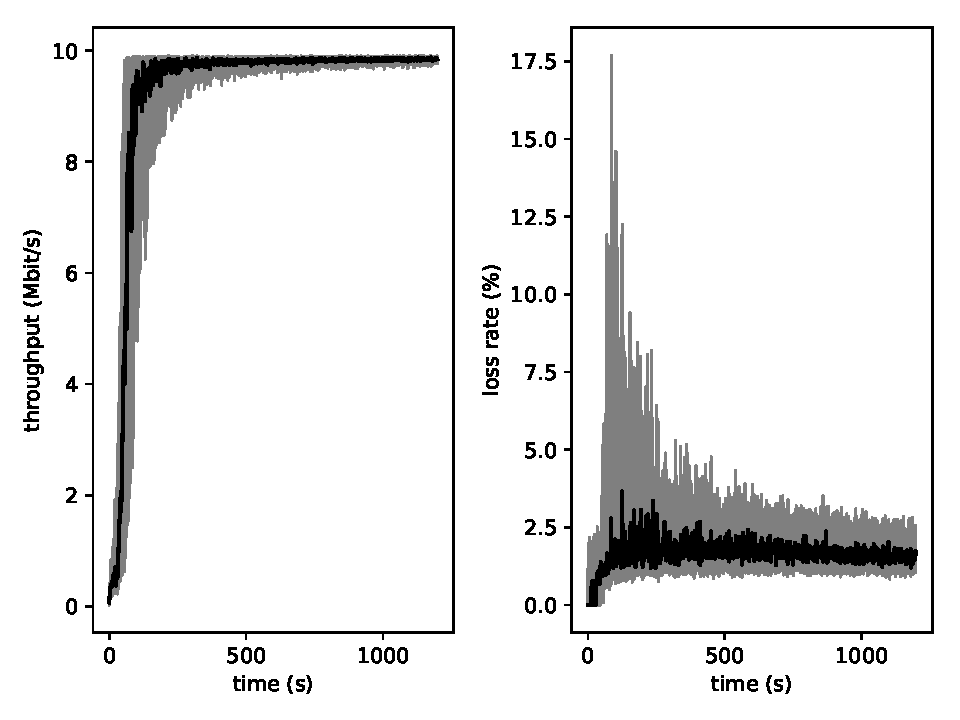
\includegraphics[width=\columnwidth]{{{/home/max/repos/remy/compute-0-4.local/figures/1_1}}}
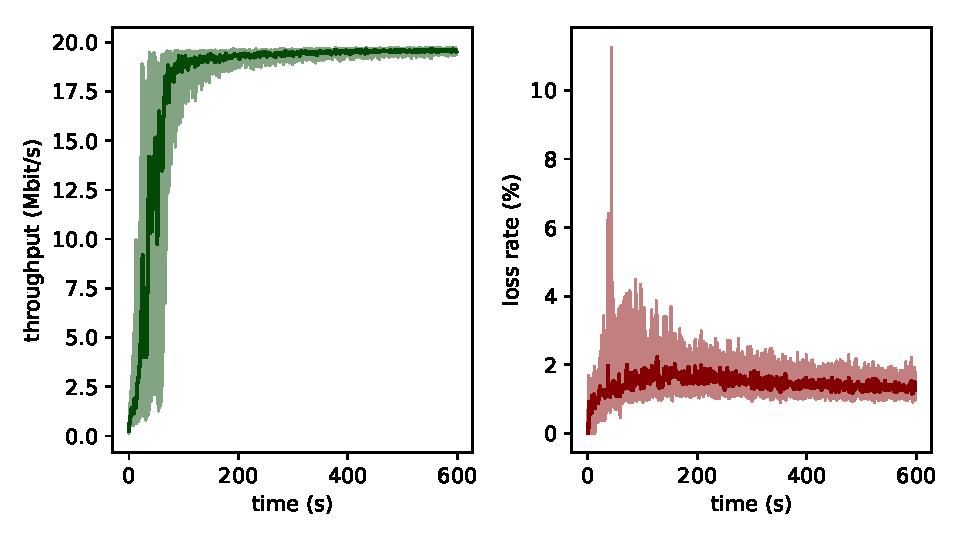
\includegraphics[width=\columnwidth]{{{/home/max/repos/remy/compute-0-4.local/figures/1_2}}}
\includegraphics[width=\columnwidth]{{{/home/max/repos/remy/compute-0-4.local/figures/1_4}}}
\caption{One sender with a bandwidth/packet loss tradeoff of 1, 2 and 4 (from top to bottom) on a link with 20\,Mbit/s bottleneck speed and 50\,ms RTT and a $\frac{1}{10}$ bandwidth delay buffer. Median in black and $\frac{1}{4}$ and $\frac{3}{4}$ quantile band in gray.}
\label{fig:one_sender_loss}
\end{minipage}
\end{figure}

The tunable tradeoff between bandwidth and packet loss rate ($\alpha$) has a clear impact on both the highest spike of packet loss that is produced in the very beginning of the online learning process as well as on the median packet loss rate later on in the learning process \autoref{fig:one_sender_loss}. However, the stronger packet loss is punished, the longer it takes for the sender to reach the maximum bandwidth on the link. 

\subsection{Number of senders}

\begin{figure}
\begin{minipage}{\columnwidth}
\includegraphics[width=\columnwidth]{{{/home/max/repos/remy/compute-0-4.local/figures/1_4}}}
\includegraphics[width=\columnwidth]{{{/home/max/repos/remy/compute-0-6.local/figures/2_4}}}
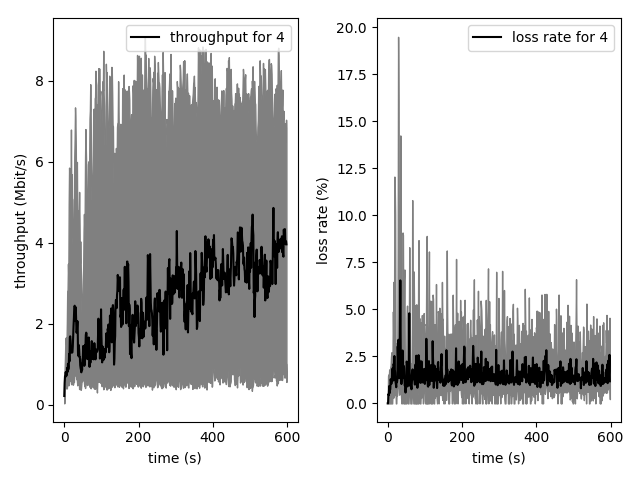
\includegraphics[width=\columnwidth]{{{/home/max/repos/remy/new_gpu/no_loss/figures/4_4}}}
\caption{One, two and four senders (from top to bottom) with a bandwidth/packet loss tradeoff of 4 on a link with 20\,Mbit/s bottleneck speed and 50\,ms RTT and a $\frac{1}{10}$ bandwidth delay buffer. Median in black and $\frac{1}{4}$ and $\frac{3}{4}$ quantile band in gray.}
\label{fig:multiple_senders}
\end{minipage}
\end{figure}

While TCP Rax generally does not exhibit much variance after a few minutes of training when it is the only flow on a link, fluctuations clearly increase when having two or four concurrent senders \autoref{fig:multiple_senders}. We attribute this to the fact that on a shared link with $n$ senders each can only get $\frac{1}{n}$ of the bandwidth on average and thus each sender receives fewer packets which he can use for training. Furthermore, as the environment becomes more dynamic with more senders, each sender has a harder time learning whether the reward changed due to his own actions or due to actions that were caused by other senders: If there is only one flow on a link, the flow ``can be sure'' that all changes in rewards were actually caused by his own actions. 

\subsection{Pre-training}

\begin{figure}
\begin{minipage}{\columnwidth}
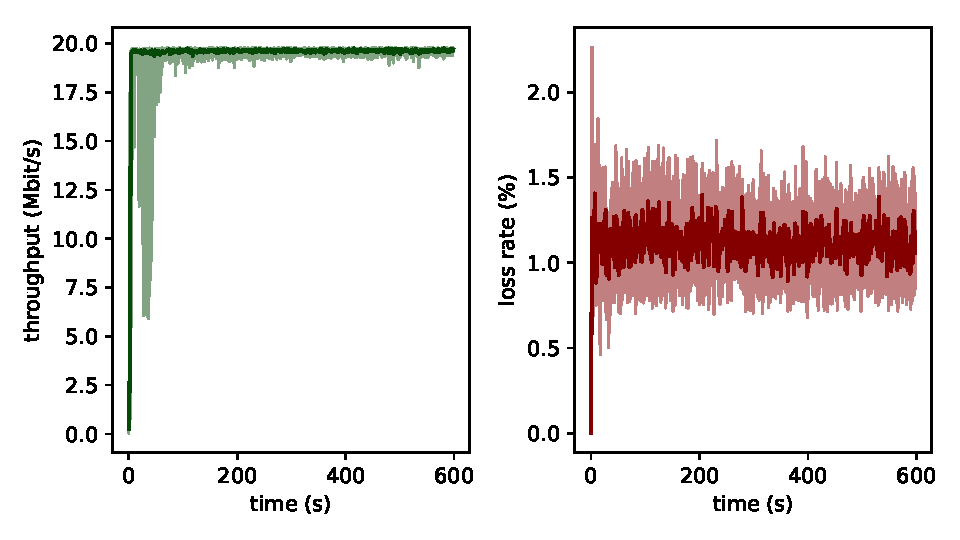
\includegraphics[width=\columnwidth]{{{/home/max/repos/remy/compute-0-4.local/figures/1_4_again}}}
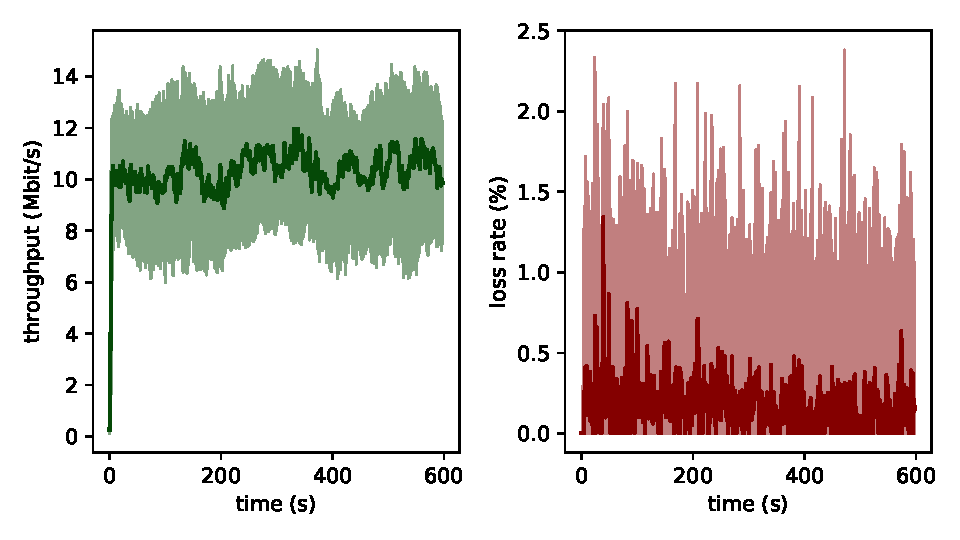
\includegraphics[width=\columnwidth]{{{/home/max/repos/remy/compute-0-6.local/figures/2_4_again}}}
\caption{One and two senders (from top to bottom) that were trained with a bandwidth/packet loss tradeoff of 2 on a link with 20\,Mbit/s bottleneck speed and 50\,ms RTT and a $\frac{1}{10}$ bandwidth delay buffer. Median in black and $\frac{1}{4}$ and $\frac{3}{4}$ quantile band in gray.}
\label{fig:resuming_training}
\end{minipage}
\end{figure}

To verify whether pre-training is generally feasible, we used the neural networks that were produced after each 600 seconds flow shown in figure \autoref{fig:multiple_senders} and started flows of equal length with the pre-trained neural networks. The flows seem to simply resume where they ended training in the flow before. This does not seem like a remarkable finding, however, this is unexpected: For instance, in the case of one sender on a link, the neural network starts with random weights and discovers that it achieves optimum utility at a window that results in 20\,Mbit/s of bandwidth. Then the sender constantly stays in this state and one would expect it to slowly ``forget'' what it learned in the very beginning when it started the flow. Thus, it is interesting that after hundreds of seconds of only seeing one same state, the neural network still acts correctly when starting with a small congestion window again in a completely different state than it is used to. 

\subsection{Stochastic Loss}

\begin{figure}
\begin{minipage}{\columnwidth}
\includegraphics[width=\columnwidth]{{{/home/max/repos/remy/compute-0-5.local/figures/1_4}}}
\includegraphics[width=\columnwidth]{{{/home/max/repos/remy/compute-0-7.local/figures/2_4}}}
\caption{One and two senders (from top to bottom) on a link with a stochastic loss rate of 1\%, a bandwidth/packet loss tradeoff of 2 on a link with 20\,Mbit/s bottleneck speed and 50\,ms RTT and a $\frac{1}{10}$ bandwidth delay buffer. Median in black and $\frac{1}{4}$ and $\frac{3}{4}$ quantile band in gray.}
\label{fig:stochastic_loss}
\end{minipage}
\end{figure}

To see whether pre-training is generally feasible, we used the neural networks that were produced after each 600 seconds flow shown in figure \autoref{fig:multiple_senders} and started flows of equal length with the pre-trained neural networks. The flows seem to simply resume where they ended training in the flow before. This does not seem like a remarkable finding, however, this is unexpected: For instance, in the case of one sender on a link, the neural network starts with random weights and discovers that it achieves optimum utility at a window that results in 20\,Mbit/s of bandwidth. Then the sender constantly stays in this state and one would expect it to slowly ``forget'' what it learned in the very beginning when it started the flow. Thus it is interesting that after hundreds of seconds of only seeing one same state, the neural network still acts correctly when starting with a small congestion window again. 

\section{Discussion}

\subsection{Best practices for on-line reinforcement learning}

\section{Conclusion}

\section*{Appendix}

\begin{algorithm}[H]
\caption{Partial Action Learning -- pseudocode for each agent. It is possible that the agents share the global weights $\theta_{\text{g}}$, which is reasonable when learning off-line. Otherwise an individual copy of them is kept by each agent. By default, all weights are initialized randomly in the beginning but it is also possible to use a pre-trained neural network for initialization. As we use Gated Recurrent Units (GRUs) their output is stored in $h$ and fed into them at the next time step.}
\label{alg:pal}
\begin{algorithmic}[1]
\Loop
	\State $l_\text{actions} \gets  [] $
	\State $l_\text{states} \gets  [] $
	\State $l_\text{values} \gets  [] $
	\State $l_\text{rewards} \gets  [] $
	\State $l_\text{values'} \gets  [] $
	\State $l_\text{snapshots} \gets  [] $
	\State $l_\text{hiddenStates} \gets  [] $
	\State $t \gets 0$
	\State $s_0 \gets \text{initialState}()$
	\State $h \gets \text{zeros}()$
	\State $\theta \gets \theta_{\text{g}}$
	\Repeat
		\State $l_\text{values'}.\text{append}(V(s_t; \theta))$
		\If{\Call{updateWeights?}{}}
			\State $\theta_\text{a} \gets \theta_{\text{g}}$
			\State $l_\text{snapshots}.\text{append}(\theta)$
			\State $l_\text{hiddenStates}.\text{append}(h)$
		\EndIf
		\State $l_\text{states}.\text{append}(s_t)$
		\State Sample $a_t$ from the 
		\StateIndent[3] Actor Network's probability distribution
		\State $l_\text{actions}.\text{append}(a_t)$
		\State $l_\text{values}.\text{append}(V(s_t; \theta_\text{v}))$ 
		\Comment{Possibly different from the}
		\StateIndent[3] value in $l_\text{values'}$ as the weights could have 
		\StateIndent[3] been updated in the meantime.
		\State $l_{\text{partialActions},t} \gets \text{partialActions}(a_t)$
		\ForAll{partial actions $a_{{\text{p},i,t}}$ in $l_{\text{partialActions},t}$}
			\State Take partial action $a_{{\text{p},i,t}}$
		\EndFor
		\State Wait for the next feedback $r_{\text{p},j,t'}$
		\StateIndent[3] where $t' \leq t$ and $0 \leq j \leq\#(l_{\text{partialActions},t'})$
		\If{all feedback of $a_{t'}$ was received}
			\State $r_{t'} \gets \text{reward w.r.t all feedback }r_{\text{p},k,t'}$
					\StateIndent[4] where $0 \leq k \leq\#(l_{\text{partialActions},t'})$
			\State $l_\text{rewards}.\text{append}(r_{t'})$
			\If{\Call{gotEnoughRewards?}{} or the episode is over}
%			\If{$\#\left(l_\text{rewards}\right) > t_\text{max}$ or the episode is over}
				\State \Call{computeGradients}{}
			\EndIf
		\EndIf
		\State Generate $s_{t+1}$ using $r_{\text{p}_{t'}}$
		\State $t \gets t+1$
	\Until{reaching the end the episode}
\EndLoop
%\algstore{palalg}
\end{algorithmic}
\end{algorithm}

\begin{algorithm}[H]
\caption{Partial Action Learning -- procedure which computes and applies the gradients.}
\label{alg:grad}
\begin{algorithmic}[1]%
%\algrestore{palalg}
\Function{computeGradients}{}
	\State $t_\text{end} = \#\left( l_\text{rewards} \right)$
	\State $\theta_\text{backup} \gets \theta$
	\State $h_\text{backup} \gets h$
	\State $\theta \gets l_\text{snapshots}[0]$
	\State $h \gets l_\text{hiddenStates}[0]$
	\State $R_{i+1} \gets$ last element of $l_\text{values'}$%
	\For{$i\gets t_\text{end}-1..0$}
		\State $R_i \gets \left(r_i + \gamma R_{i+1}\right)\left(1-\gamma\right)$
		\State $a \gets l_\text{actions}[i]$
		\State $s \gets l_\text{states}[i]$
		\State $v \gets l_\text{values}[i]$
		\State $d\theta \gets -\frac{\partial\log \left( \pi\left( a \given s; \theta_\text{a} \right)\right)\left(R_i - v\right)}{\partial\theta}$
		\StateIndent[4] $-\frac{\partial\beta H\left( \pi\left( s; \theta_a \right)\right)}{\partial\theta}$
		\StateIndent[4] $+\frac{\partial\left(R_i - v\right)}{\partial\theta}$
		\State $\theta_{\text{g}} \gets \theta_{\text{g}} + d\theta$
	\EndFor
	\State Remove first $t_\text{end}$ elements from
	\StateIndent[2] $l_\text{actions}$, $l_\text{states}$, $l_\text{values}$, $l_\text{rewards}$, $l_\text{values'}$
	\State Remove the first element from $l_\text{snapshots}$
	\State Remove the first element from $l_\text{hiddenStates}$
	\State $\theta = \theta_\text{backup}$
	\State $h = h_\text{backup}$
\EndFunction
\end{algorithmic}
\end{algorithm}

\begin{algorithm}[H]
\caption{Procedure which determines when to synchronize the neural network weights from the global weights in case of congestion control. We assume that the window at time step $t$ is stored in a list $l_\text{windows}$ and that the number of bytes sent in each time step is stored in $l_\text{sent}$. Alternatively to this procedure one can simply synchronize the weights after each $t_\text{max}$ actions where $t_\text{max}$ is an arbitrarily chosen integer greater than 0.}
\label{alg:update}
\begin{algorithmic}[1]%
%\algrestore{palalg}
\Function{updateWeights?}{}
	\State $i \gets 0$
	\While{$i < \#(l_\text{actions})$}
		\State $w\gets \left\lfloor l_\text{windows}[i] + l_\text{actions}[i] \right\rfloor $
		\For{$j\gets i..\#(l_\text{actions})-1$}
			\State $w\gets \text{w} - l_\text{sent}[j]$
			\If{$w\leq 0 \land i+1 \geq 10$} \Comment{at least 10 rewards}
				\State $i \gets j$
				\State \Break
			\EndIf
		\EndFor
		\If{$i = \#(l_\text{windows})-1$}
			\State \Return \True
		\EndIf
	\EndWhile
	\State \Return \False
\EndFunction
\end{algorithmic}
\end{algorithm}

\begin{algorithm}[H]
\caption{Procedure which determines when to start computing the gradients in case of congestion control. We assume that the window at time step $t$ is stored in a list $l_\text{windows}$ and that the number of bytes sent in each time step is stored in $l_\text{sent}$. Alternatively to this procedure one can simply compute the gradients when $t_\text{max}$ rewards have been received where $t_\text{max}$ is an arbitrarily chosen integer greater than 0.}
\label{alg:enough}
\begin{algorithmic}[1]%
%\algrestore{palalg}
\Function{gotEnoughRewards?}{}
	\State $w \gets \left\lfloor l_\text{windows}[0] + l_\text{actions}[0] \right\rfloor$
	\For{$i\gets 0..\#(l_\text{rewards})-1$}
		\State $w \gets \text{w} - l_\text{sent}[i]$
		\If{$w \leq 0 \land i+1 \geq 10$} \Comment{at least 10 rewards}
			\State \Return \True
		\EndIf
	\EndFor
	\State \Return \False
\EndFunction
\end{algorithmic}
\end{algorithm}

%\subsection{Convergence}
%
%We use 
%
%\begin{align*}
%\text{Reward} = \log(\text{throughput}) - \delta\text{delay}
%\end{align*}
%
%as our metric of reward, where $\delta$ is a parameter that allows us to change the importance of the throughput vs.~the delay. We take the logarithm of the throughput to ensure that flows which have small throughput have a higher incentive to increase it as flows which already have a large one (because the derivative of the logarithm decreases with increasing value). We take minus the delay to punish inducing delay. We do not take the logarithm because we think that it is equally bad if a sender behind a satellite connection with a minimum RTT of $500\,$ms adds $1\,$ms of delay as if a sender connected using Ethernet with a minimum RTT of $10\,$ms adds $1\,$ms of delay. 
%
%There are two conditions that we have to take into account to ensure convergence:
%\begin{enumerate}
%\item \begin{align*}
%\left(\frac{\partial}{\partial w}\text{throughput}\right)\left(1\right) > \left(\frac{\partial}{\partial w}\delta\text{delay}\right)\left(1\right)
%\end{align*}
%\item \begin{align*}
%\frac{\partial}{\partial w}\left(\delta\right)
%\end{align*}
%\end{enumerate}
%
%\todo{Finish second constraint for convergence.}
%
%\todo{Add figure to visually explain that}

%\subsection{Convergence}
%
%Assume we have $N$ senders, each with its specific baseline delay (this encompasses all delays excluding only the queueing delay) $d_i$. Each sender keeps a congestion window $b_i$. The link speed at the bottleneck is designated as $c$. 
%
%%We define the excessive window as 
%%\begin{align*}
%%b_\text{excess} = \max\left( \left( \sum_{j=1}^N \frac{b_j}{d_j} \right) - c, 0 \right)
%%\end{align*}
%%and the queueing delay as 
%%\begin{align*}
%%d_q = \frac{b_\text{excess}}{c}.
%%\end{align*}
%
%With $b = (b_i)$ we observe the following relation:
%
%\begin{align*}
%c = \sum_{j=1}^N \frac{b_j}{d_j + d_q(b)}
%\end{align*}
%
%Then we define the utility function for each sender $i$ as
%\begin{align*}
%V_i(b) \coloneqq \begin{cases}
%\log\left(\frac{b_i}{d_i}\right) - \delta_i d_i & \text{if } \sum_{j=1}^N \frac{b_i}{d_i} \leq c\\
%\log\left(\frac{b_i}{d_i + d_q(b)}\right) - \delta_i (d_i + d_q(b)) & \text{otherwise}
%\end{cases}
%\end{align*}
%
%\begin{align*}
%&\log\left(\frac{b_i}{d_i + d_q}\right) - \delta_i (d_i + d_q) \\
%=& \log\left(b_i\right) - \log\left(d_i + d_q\right) - \delta_i (d_i + d_q)
%\end{align*}
%
%\begin{align*}
%\frac{\partial V_i}{\partial b_i} = \begin{cases}
%\frac{1}{b_i} & \text{if } \sum_{j=1}^N \frac{b_i}{d_i} \leq c\\
%\frac{1}{b_i} - \frac{\partial d_q}{\partial b_i}\left(b_i\right)\frac{1}{d_i+d_q\left(b_i\right)} - \delta\frac{\partial d_q}{b_i}\left(b_i\right) & \text{otherwise}
%\end{cases}
%\end{align*}

%\begin{align*}
%G(b) = \begin{pmatrix}
%-\frac{1}{b_1^2} & & \\
%& \ddots & \\
%& & -\frac{1}{b_N^2}
%\end{pmatrix} \text{if } \text{if } \sum_{j=1}^N \frac{b_i}{d_i} \leq c
%\end{align*}

%To show diagonal strict concavity we have to show that d.s.c.~is fulfilled \begin{enumerate*} \item for two distinct points lying in $\sum_{j=1}^N \frac{b_i}{d_i} \leq c$ \item for two distinct points lying in $\sum_{j=1}^N \frac{b_i}{d_i} > c$ and \item when one point is in one part of the function and the other in the other one\end{enumerate*}.
%
%\todo{Insert what d.s.c~actually is and quote Altman's paper}

%\begin{enumerate}
%\item (b^1 - 
%\item
%\item
%\end{enumerate}

%\section{Results}
%
%We train on the following scenario:
% 
%\begin{table}[h]
%\centering
%\begin{tabular}{rll}
%\toprule
%Parameter & Value & Distribution \\
%\midrule
%Two-way propagation delay & $100\,$ms & constant \\
%Bottleneck bandwidth & $3\,$Mbit/s & constant \\
%Number of senders & $2$ & constant \\
%Flow length & $\infty$ & constant \\
%Simulation duration & $50\,$s--$150\,$s & uniform \\
%Buffer size & $\infty$ & constant \\
%Stochastic loss prob. & $0\%$ & constant \\
%\bottomrule
%\end{tabular}
%\caption{The parameters of our very first simple experiment}
%\label{tab:smallexperiment}
%\end{table}
%
%\todo{Insert results when comparing to regular TCP}
 
\bibliographystyle{ACM-Reference-Format}
\bibliography{congestion}

\end{document}
